\documentclass[hyperref=colorlinks]{beamer}
\mode<presentation>
\usetheme{iclpt}
\setbeamertemplate{navigation symbols}{}
\setbeamertemplate{headline}{
\begin{beamercolorbox}[leftskip=.2cm,rightskip=.2cm,topskip=.2cm,ht=1.1cm,dp=0.1cm,wd=\textwidth]{institute in head/foot}
  
\includegraphics[height=1cm]{icl.pdf}
  \hfill
  
\includegraphics[height=1cm]{../Pics/CMS-Color.pdf}
\end{beamercolorbox}
}
\setbeamertemplate{footline}{
\begin{beamercolorbox}[ht=.55cm,dp=0.4cm,wd=\textwidth,leftskip=.3cm]{author in head/foot}%
  \begin{minipage}[c]{5cm}%
    \usebeamerfont{author in head/foot}
    \insertshortauthor 
    \insertshorttitle
    \end{minipage}\hfill%
  \insertframenumber{} / \pageref{lastframe}
  \hfill
  \begin{minipage}{6cm}
    \hfill
  \end{minipage}
\end{beamercolorbox}%
}

\usepackage{color}
\usepackage{tabularx,colortbl}
\usepackage{graphicx}
\usepackage{pdfpages}
\usepackage{feynmp}
\usepackage{multirow}
\DeclareGraphicsRule{*}{mps}{*}{}

\title{\vspace{-0.2cm} Higgs to Invisible Combination - Approval}
\subtitle{This result: HIG-15-012 \\ Contributing analyses: HIG-13-030, HIG-14-038, EXO-12-055}
\author[P. Dunne]{\underline{P. Dunne} on behalf of the H$\rightarrow$invisible analysis groups}
\titlegraphic{
  \vspace{-0.7cm}
  %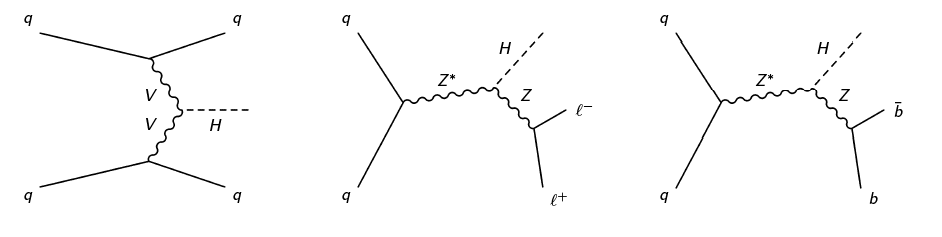
\includegraphics[width=\textwidth]{TalkPics/invcomb021213/feyndiags}
%% \begin{fmfgraph*}(100,70)
%%         \fmfleft{i1,i2}
%%         \fmfright{o1,o2,o3}
%%         \fmf{fermion}{i1,v1,o1}
%%         \fmf{fermion}{i2,v2,o3}
%%         \fmf{phantom,tension=4/5}{v1,v2}
%%         \fmffreeze
%%         \fmf{photon,label=$W,,Z$}{v1,v3}
%%         \fmf{photon,label=$W,,Z$}{v2,v3}
%%         \fmf{dashes}{v3,o2}
%%         \fmflabel{$q$}{i1}
%%         \fmflabel{$q$}{i2}
%%         \fmflabel{$q$}{o1}
%%         \fmflabel{$q$}{o3}
%%         \fmflabel{$H$}{o2}
%%       \end{fmfgraph*}
}
\date{}
\begin{document}
\begin{fmffile}{hig15012preapprovalfeyndiags}

%TITLE PAGE
\section{Title}
\begin{frame}
  \titlepage
  
\end{frame}

%!!CLOSURE TEST STATEMENT PU jet ID
%OUTLINE
\begin{frame}
      \scriptsize
  \begin{columns}
    \column{.65\textwidth}
    \vspace{-.2cm}
    \begin{block}{\footnotesize Reminder}
      \begin{itemize}
      \item Run 1 Prompt data searches in  Z($\ell\ell$)H, Z(bb)H and VBF channels published in HIG-13-030
      \item VBF updated with parked data in HIG-14-038
      \item EXO-12-055 targeting V(had)H and ggH production
      \item Motivation:
      \item[-] Uncertainties on Higgs measurements can still accommodate significant BSM properties
      \item[-] Many BSM theories predict H$\rightarrow$ invisible
      \end{itemize}
    \end{block}
    \vspace{-.2cm}
    \begin{block}{\footnotesize Overview}
      \scriptsize
      \begin{itemize}
      \item Reminder of contributing analyses
%      \item Details of combination:
%      \item[-] Overlap between HIG-14-038 and EXO-12-055
%      \item[-] Correlation of uncertainties
      \item Combination reminder and items raised by ARC
      \item Unblinded results and plots for approval
      \end{itemize}
    \end{block}
    \column{.45\textwidth}
    \centering
    \begin{fmfgraph*}(80,50)
      \fmfleft{i1,i2}
      \fmfright{o1,o2,o3}
      \fmf{fermion}{i1,v1,o1}
      \fmf{fermion}{i2,v2,o3}
      \fmf{phantom,tension=4/5}{v1,v2}
      \fmffreeze
      \fmf{photon}{v1,v3}
      \fmf{photon}{v2,v3}
      \fmf{dashes}{v3,o2}
      \fmflabel{$q$}{i1}
      \fmflabel{$q$}{i2}
      \fmflabel{$q$}{o1}
      \fmflabel{$q$}{o3}
      \fmflabel{$H$}{o2}
    \end{fmfgraph*}

    \vspace{.6cm}

    \begin{fmfgraph*}(80,50)
      \fmfleft{i1,i2,ix,i3,iy,i4,i5}
      \fmfright{o1,o2,ox,o3,oy,o4,o5}
      \fmf{phantom}{i2,v1,o2}
      \fmf{phantom}{i4,v2,o4}
      \fmffreeze
      \fmf{gluon}{i2,v1}
      \fmf{gluon}{i4,v2}
      \fmf{phantom}{v1,v4,v3,v5,v2,v1}
      \fmf{fermion}{v1,v3,v2,v1}
      \fmf{dashes,tension=8/5}{v3,o3}
      \fmffreeze
      \fmf{gluon}{v4,o2}
      \fmflabel{$g$}{i2}
      \fmflabel{$g$}{i4}
      \fmflabel{$H$}{o3}
      \fmflabel{$jet$}{o2}
    \end{fmfgraph*}

    \vspace{.6cm}

    \begin{fmfgraph*}(80,50)
      \fmfleft{i1,i2}
      \fmfright{o1,o2,o3}
      \fmf{fermion}{i1,v1,i2}
      \fmf{photon}{v1,v2,o1}
      \fmf{dashes}{v2,o3}
      \fmflabel{$q$}{i1}
      \fmflabel{$q$}{i2}
      \fmflabel{$Z$}{o1}
      \fmflabel{$H$}{o3}
    \end{fmfgraph*}

    
    \end{columns}
\end{frame}

\section{Analyses}
\begin{frame}[c]
  \begin{center}
    \Huge \color{beamer@icmiddleblue}{Analyses}
  \end{center}
\end{frame}

\begin{frame}
  \frametitle{VBF - HIG-14-038, AN-2014/243}
  \begin{columns}
    \column{.6\textwidth}
    \scriptsize
    \begin{block}{Strategy}
      \begin{itemize}
      \item Select 2 jets with large $\Delta\eta$ + MET
      \item Remove QCD with tight selection
      \item Use data driven methods to estimate major backgrounds
      \end{itemize}
    \end{block}
    \begin{block}{Signal extraction and results}
      \begin{itemize}
      \item Single bin counting experiment
      \item 95\% CL observed (expected) limit on B(H$\rightarrow$inv) 57(40)\%
      \end{itemize}
    \end{block}
    \column{.45\textwidth}
    \centering

    \vspace{.1cm}

    \begin{fmfgraph*}(100,70)
      \fmfleft{i1,i2}
      \fmfright{o1,o2,o3}
      \fmf{fermion}{i1,v1,o1}
      \fmf{fermion}{i2,v2,o3}
      \fmf{phantom,tension=4/5}{v1,v2}
      \fmffreeze
      \fmf{photon,label=$W,,Z$}{v1,v3}
      \fmf{photon,label=$W,,Z$}{v2,v3}
      \fmf{dashes}{v3,o2}
      \fmflabel{$q$}{i1}
      \fmflabel{$q$}{i2}
      \fmflabel{$q$}{o1}
      \fmflabel{$q$}{o3}
      \fmflabel{$H$}{o2}
    \end{fmfgraph*}
    

    \vspace{.3cm}
    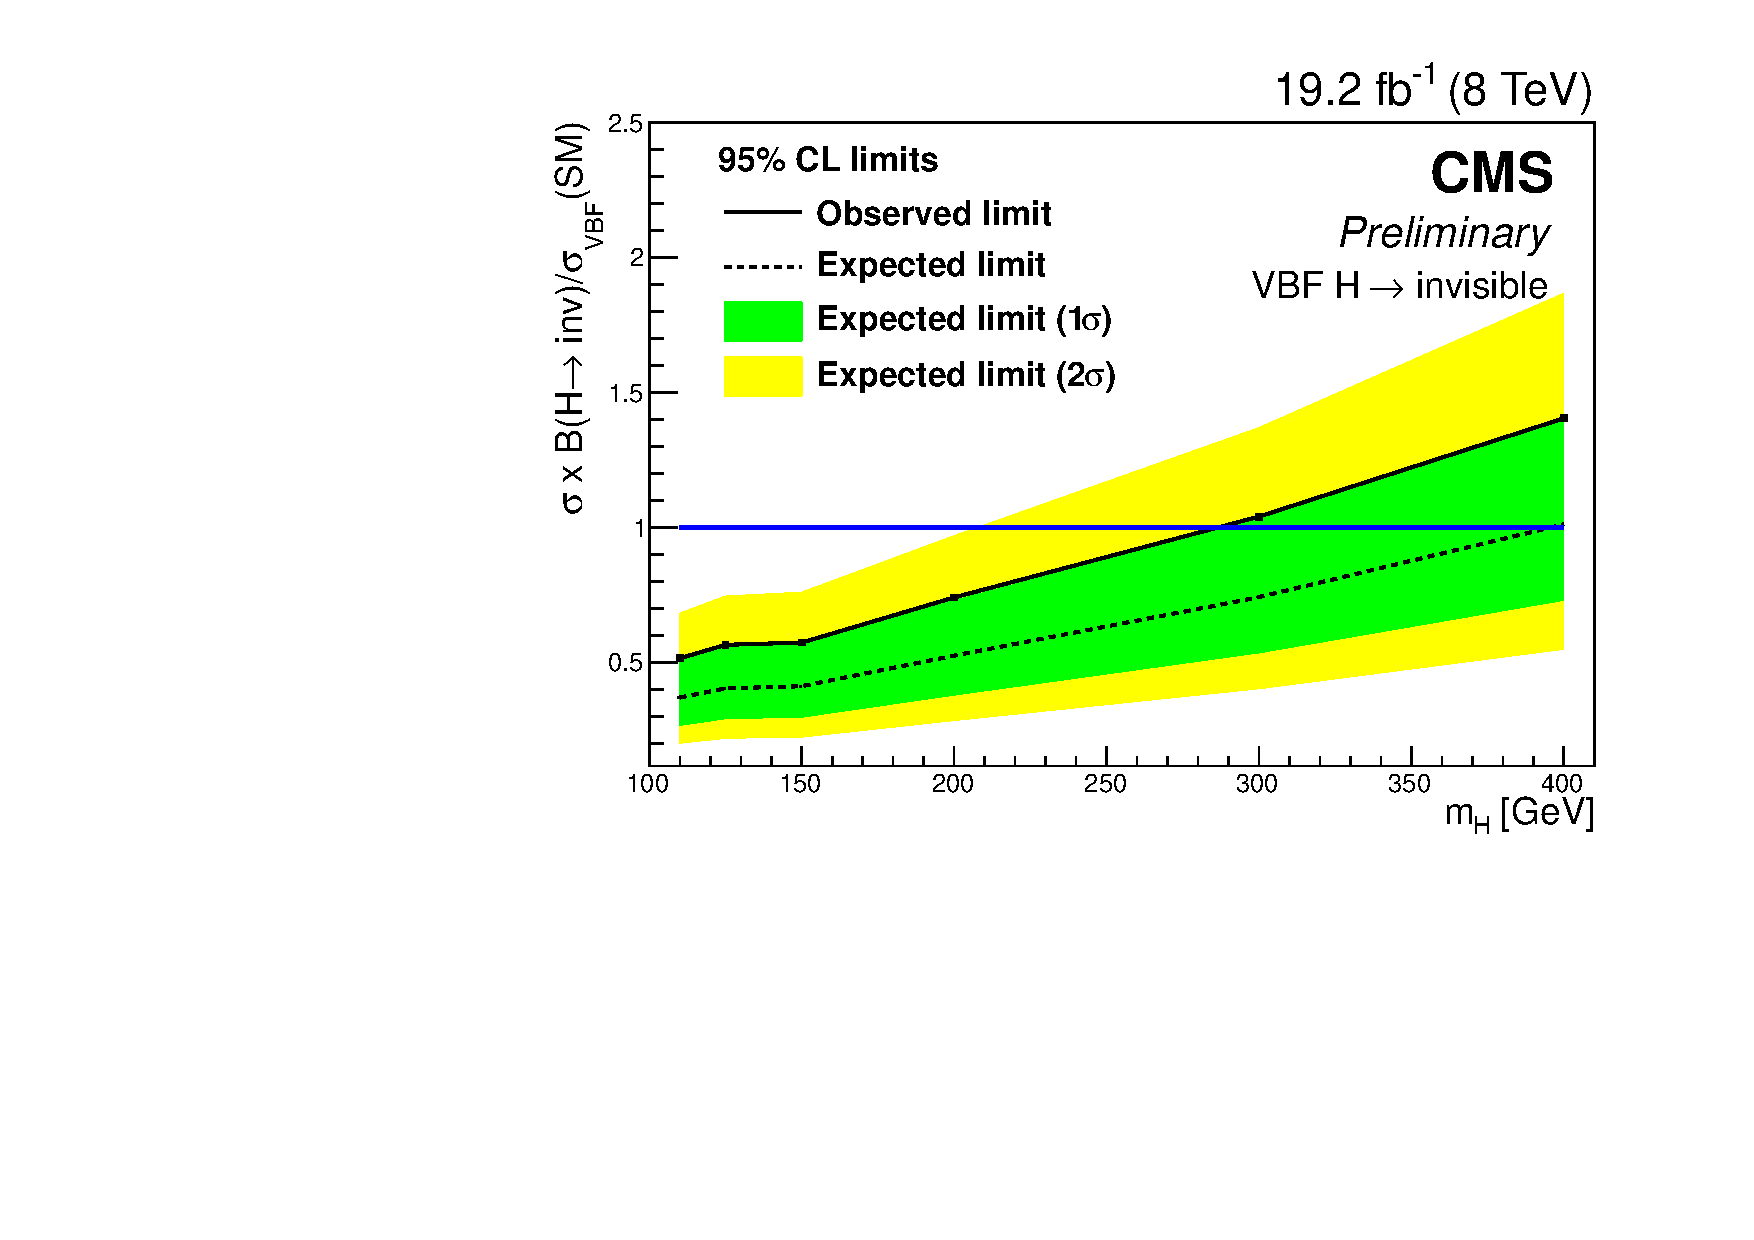
\includegraphics[width=\textwidth]{TalkPics/hig15012preapproval/VBFlim.pdf}
  \end{columns}
\end{frame}

\begin{frame}
  \frametitle{Monojet+V(had)H-tagged - EXO-12-055, AN-2014/206
}
  \scriptsize
  \begin{columns}
    \column{.6\textwidth}
    \begin{block}{Strategy}
      \begin{itemize}
      \item Select a high energy jet+MET
      \item Categorise events as boosted or resolved V-tagged or no V-tag
      \item Use data driven methods to estimate major backgrounds
      \end{itemize}
    \end{block}
    \begin{block}{Signal extraction and results}
      \begin{itemize}
      \item Simultaneous fit to MET in signal and control regions
      \item 95\% CL observed (expected) limit on B(H$\rightarrow$inv) 54(62)\%
      \end{itemize}
    \end{block}
    \column{.45\textwidth}
    \centering

    \begin{fmfgraph*}(100,70)
      \fmfleft{i1,i2,ix,i3,iy,i4,i5}
      \fmfright{o1,o2,ox,o3,oy,o4,o5}
      \fmf{phantom}{i2,v1,o2}
      \fmf{phantom}{i4,v2,o4}
      \fmffreeze
      \fmf{gluon}{i2,v1}
      \fmf{gluon}{i4,v2}
      \fmf{phantom}{v1,v4,v3,v5,v2,v1}
      \fmf{fermion}{v1,v3,v2,v1}
      \fmf{dashes,tension=8/5}{v3,o3}
      \fmffreeze
      \fmf{gluon}{v4,o2}
      \fmflabel{$g$}{i2}
      \fmflabel{$g$}{i4}
      \fmflabel{$H$}{o3}
      \fmflabel{$jet$}{o2}
    \end{fmfgraph*}

    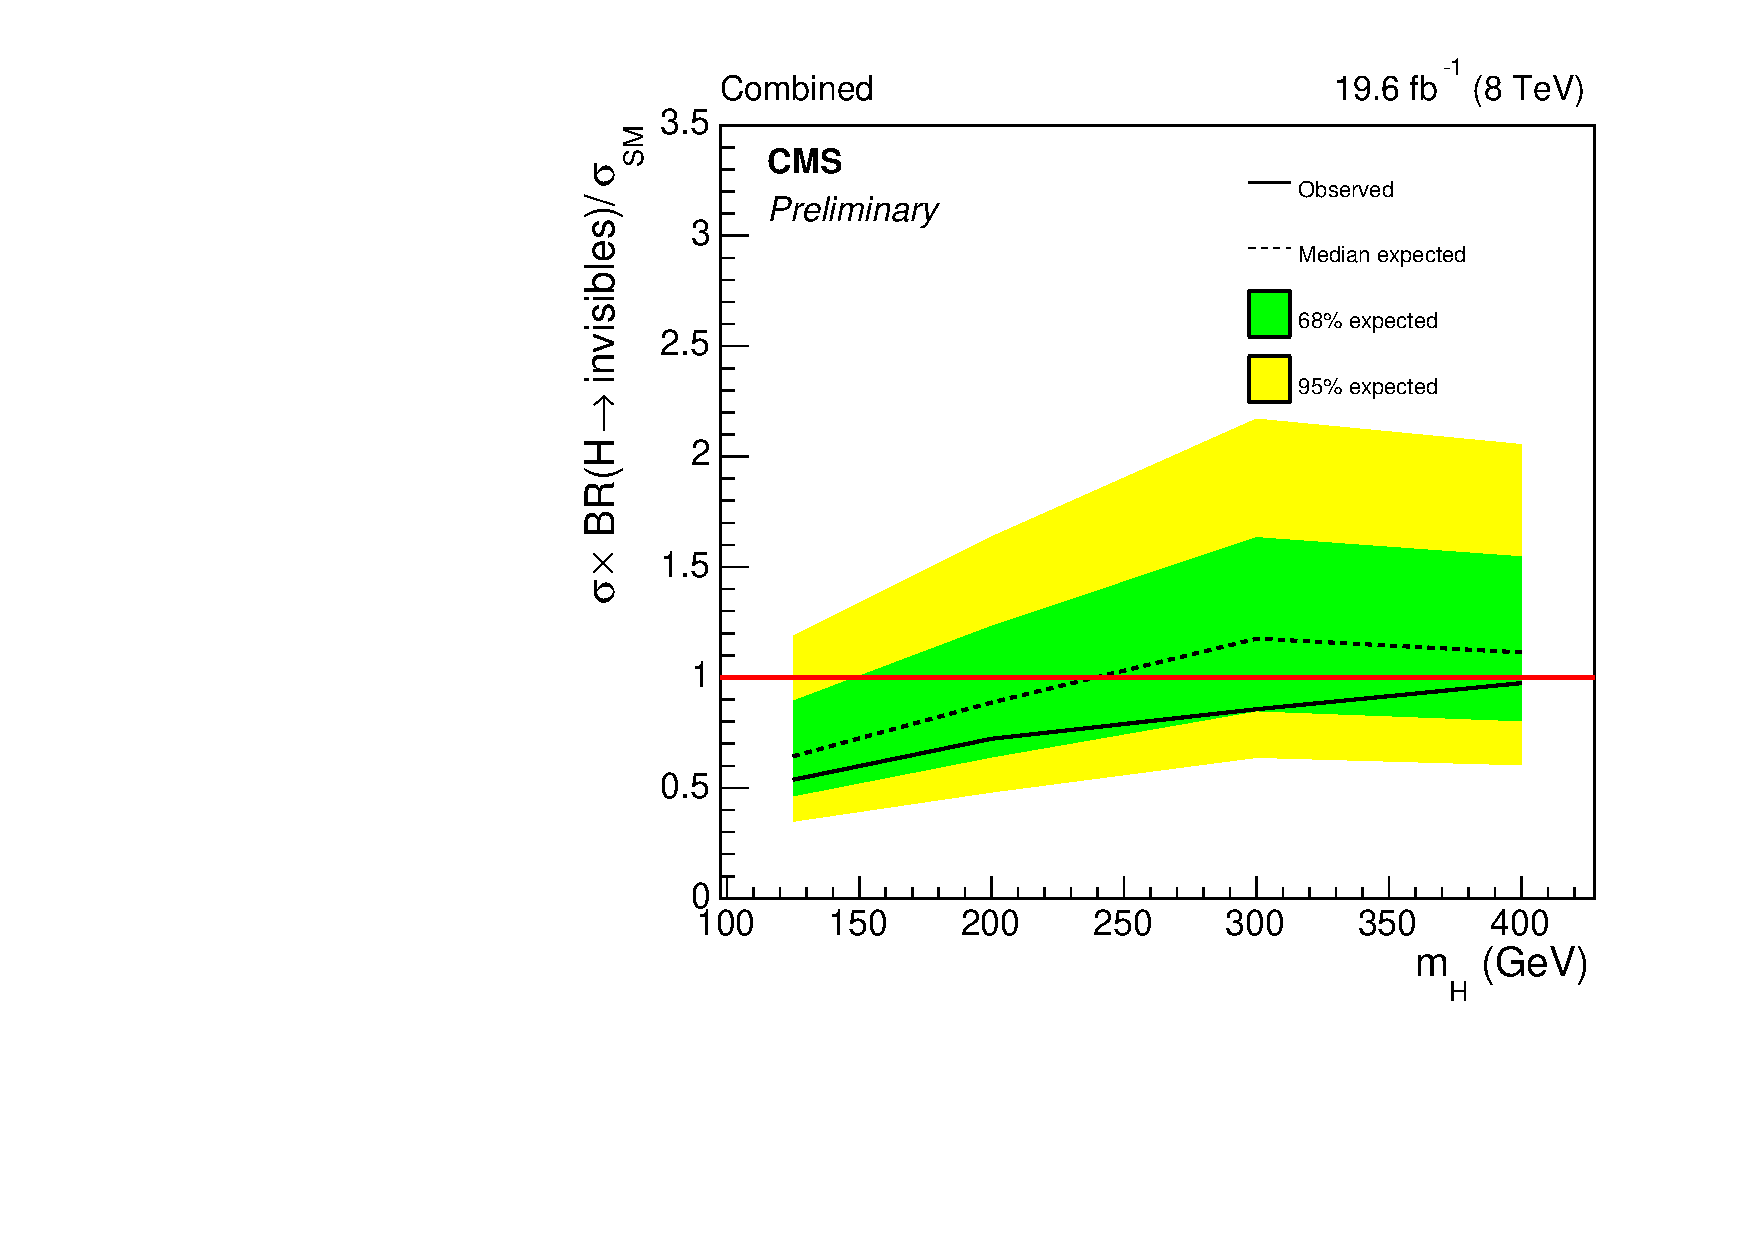
\includegraphics[width=.9\textwidth]{TalkPics/hig15012preapproval/EXOlim.pdf}
  \end{columns}
\end{frame}

\begin{frame}
  \frametitle{Z(ll)H - HIG-13-030, AN-2013/333}
  \scriptsize
  \begin{columns}
    \column{.6\textwidth}
    \begin{block}{Strategy}
      \begin{itemize}
      \item Select two electrons or muons compatible with a Z decay + MET
      \item Categorise by lepton flavour and presence of a jet
      \item Use data driven methods to estimate remaining backgrounds        
      \end{itemize}
    \end{block}
    \begin{block}{Signal extraction and results}
      \begin{itemize}
      \item 2D (1D) fit to $m_{ll}$ and $m_{T}$ ($m_{T}$) in 8 (7) TeV
      \item 95\% CL observed (expected) limit on B(H$\rightarrow$inv) 83(86)\%
      \end{itemize}
    \end{block}
    \column{.45\textwidth}
    \centering
    \begin{fmfgraph*}(100,60)
      \fmfleft{i1,i2}
      \fmfright{o1,o2,o3}
      \fmf{fermion}{i1,v1,i2}
      \fmf{photon,label=$Z$}{v1,v2,v3}
      \fmf{fermion}{o1,v3,o2}
      \fmf{dashes}{v2,o3}
      \fmflabel{$q$}{i1}
      \fmflabel{$q$}{i2}
      \fmflabel{$l$}{o1}
      \fmflabel{$l$}{o2}
      \fmflabel{$H$}{o3}
    \end{fmfgraph*}

    \vspace{.5cm}
    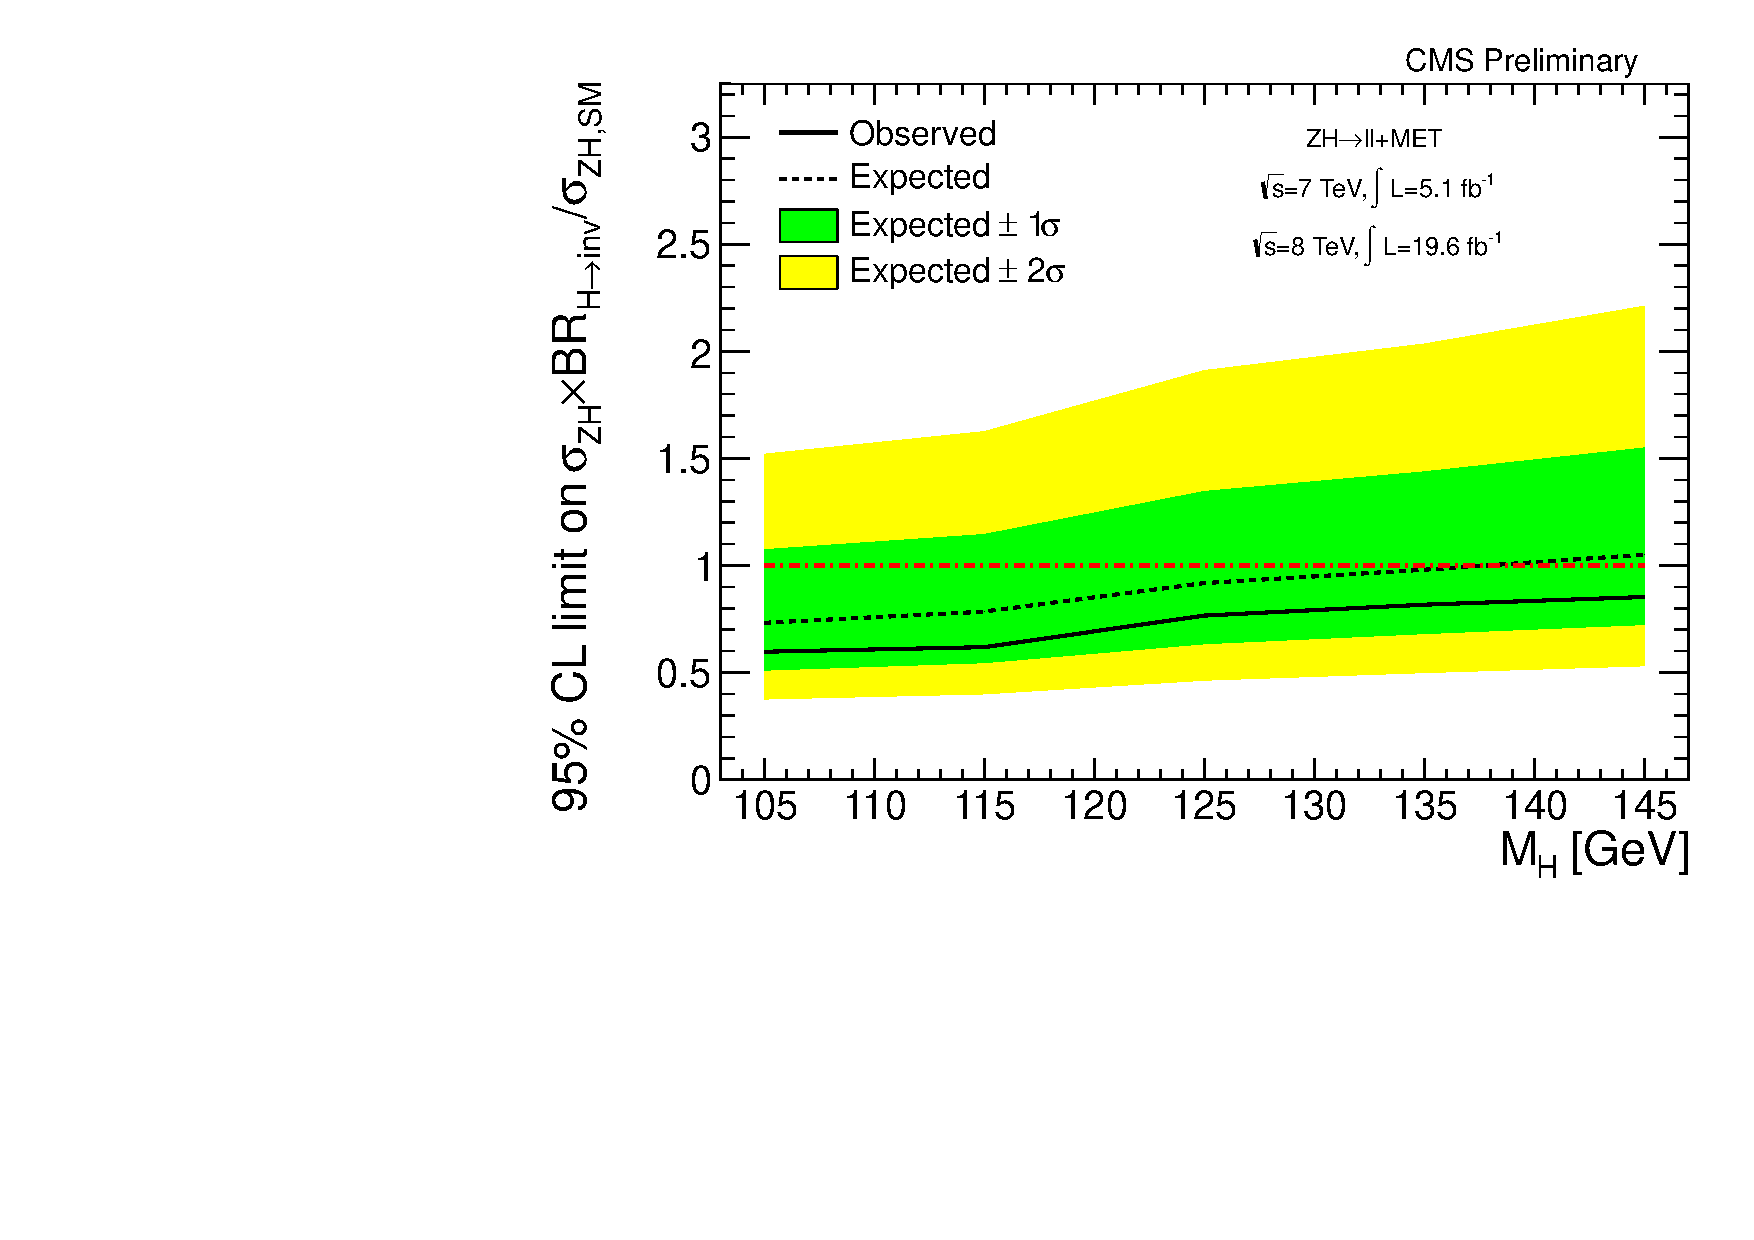
\includegraphics[width=\textwidth]{TalkPics/hig15012preapproval/ZllHlim.pdf}
  \end{columns}

\end{frame}

\begin{frame}
  \frametitle{Z(bb)H - HIG-13-030, AN-2013/222}
  \scriptsize
  \begin{columns}
    \column{.6\textwidth}
    \begin{block}{Strategy}
      \begin{itemize}
      \item Based on H(bb)Z(inv) analysis:
      \item[-] Require two jets consistent with $Z\rightarrow$bb+MET
      \item Categorise according to MET
      \item Backgrounds from MC normalised in simultaneous fit to signal and control regions
      \end{itemize}
    \end{block}
    \begin{block}{Signal extraction and results}
      \begin{itemize}
      \item Fit to BDT
      \item 95\% CL observed (expected) limit on B(H$\rightarrow$inv) 182(199)\%
      \end{itemize}
    \end{block}
    \column{.45\textwidth}
    \centering
    \begin{fmfgraph*}(100,60)
      \fmfleft{i1,i2}
      \fmfright{o1,o2,o3}
      \fmf{fermion}{i1,v1,i2}
      \fmf{photon,label=$Z$}{v1,v2,v3}
      \fmf{fermion}{o1,v3,o2}
      \fmf{dashes}{v2,o3}
      \fmflabel{$q$}{i1}
      \fmflabel{$q$}{i2}
      \fmflabel{$b$}{o1}
      \fmflabel{$\bar{b}$}{o2}
      \fmflabel{$H$}{o3}
    \end{fmfgraph*}

    \centering
    \vspace{.5cm}
    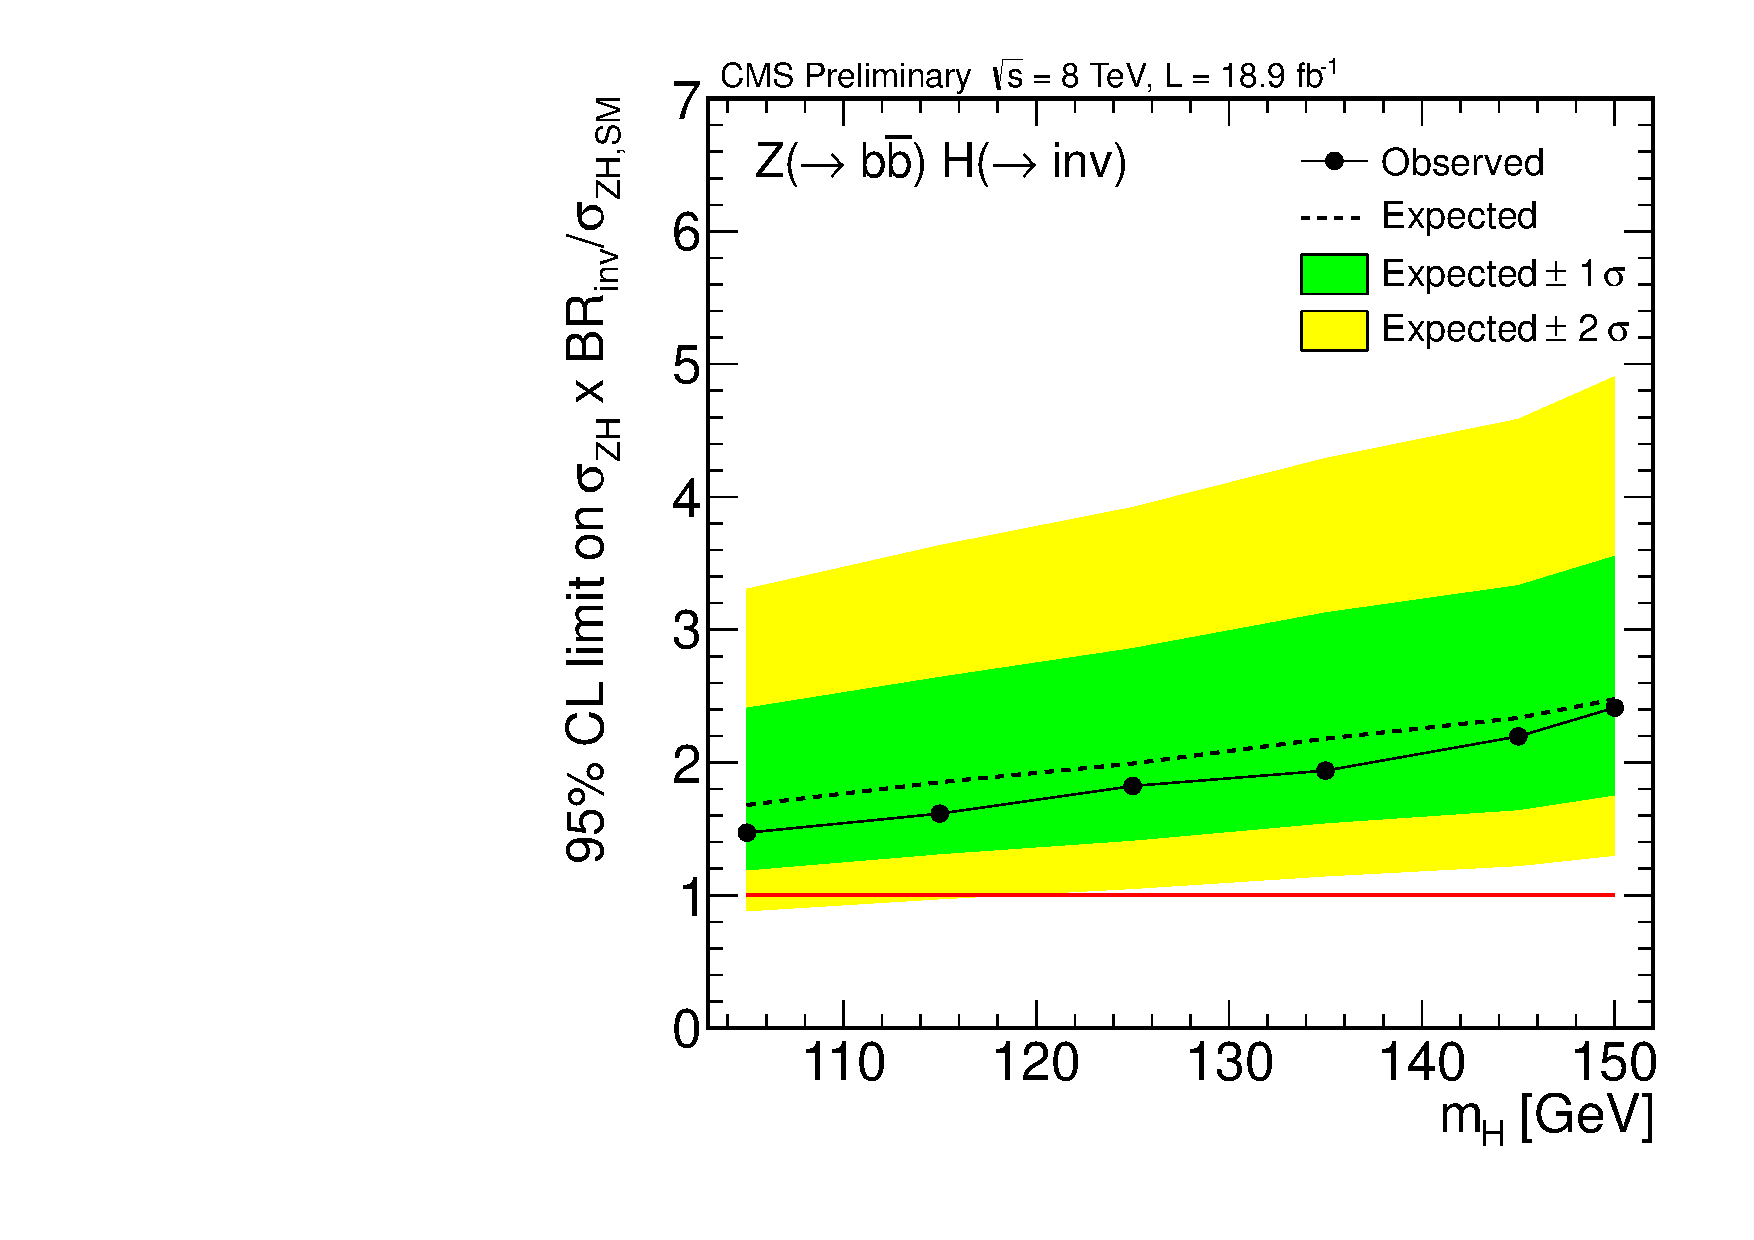
\includegraphics[width=.75\textwidth]{TalkPics/hig15012preapproval/ZbbHlim.pdf}
  \end{columns}

\end{frame}

\section{Combination Method}
\begin{frame}[c]
  \scriptsize
  \begin{center}
    \Huge \color{beamer@icmiddleblue}{Reminder of Analysis}
  \end{center}
\end{frame}

\begin{frame}
  \frametitle{Overlaps}
  \scriptsize
  \vspace{-.2cm}
  \begin{block}{\scriptsize Overlaps between VBF, Z(ll)H, Z(bb)H}
    \begin{itemize}
    \item VBF, Z(ll)H and Z(bb)H analyses are exclusive by design:
    \item[-] VBF requires no leptons and high $M_{jj}$
    \item[-] Z(ll)H requires two leptons
    \item[-] Z(bb)H requires no leptons and low $M_{jj}$
    \end{itemize}
  \end{block}
  
  \vspace{-.1cm}
  
  \begin{block}{\scriptsize Overlaps between monojet+V(had) and other analyses}
    \begin{itemize}
    \item Z(bb)H and resolved category of monojet+V(had) have potential overlap
    \item[-] Not expected to impact result
    \item[-] Completely removing resolved category has no effect on expected limit
    \item VBF and monojet+V(had)-tagged analyses do have overlap:
    \item[-] Veto events from monojet+V(had) analysis with 1st (2nd) jet with $p_{T}>$50 (45) GeV, $M_{jj}>$1200 GeV, $\eta_{j1}\cdot\eta_{j2}<0$ and $\Delta\eta_{jj}>3.6$     
    \item[-] Veto is solely for clean statistical combination not for further separation of production modes
    \end{itemize}
  \end{block}
\end{frame}

\begin{frame}
  \frametitle{Effect of VBF veto}
  \scriptsize
  \begin{columns}
    \column{1.1\textwidth}
    \begin{block}{Events rejected by VBF veto}
      \centering
      \begin{tabular}{lccc}
        \hline
        Sample & Monojet & Boosted & Resolved \\
        \hline
        \hline
        VBF & 13.2\% & 11.0\% & 0.0\% \\
        \hline
        ggH & 1.52\% & 0.0\% & 0.0\% \\
        \hline
        Data & 0.4\% & 0.2\% & 0.5\% \\
        \hline
        \hline
        Expected signal & 70\% ggH, 20\% VBF, & 47\% WH, 25\% ggH, & 39\% ggH, 32\% WH, \\
        composition & 6\% WH, 3\% ZH & 23\% ZH, 5\% VBF & 18\% ZH, 11\% VBF \\
      \end{tabular}
    \end{block}
  \end{columns}
  \begin{block}{}
    \begin{itemize}
    \item Explicitly checked overlap after veto in signal and dimuon control regions
    \item 3 out of 89,304 events found to overlap
    \item[-] All in monojet category at low MET
    \item[-] All have a 2nd jet rejected by PU ID - thought to be from small input differences
    \item Full monojet+V(had) analysis is rerun after veto:
    \item[-] All results shown are after veto
    \end{itemize}
  \end{block}

\end{frame}

\begin{frame}
  \frametitle{Correlated Nuisances}
  \scriptsize

    \begin{columns}
      \column{1.05\textwidth}
  \begin{block}{}
    \scriptsize
      \centering
    \begin{tabular}{|l|c|}
      \hline
      Nuisance & Analyses which it affects \\
      \hline
      Jet energy scale & VBF, Z($\ell\ell$)H(inv) \\
      PDF uncertainties & VBF, Z($b\bar{b}$), Z($\ell\ell$)H(inv), monojet+V(had) \\
      QCD scale & VBF, Z($b\bar{b}$), Z($\ell\ell$)H(inv), monojet+V(had) \\
      Luminosity & VBF, Z($b\bar{b}$)H(inv), Z($\ell\ell$)H(inv), monojet+V(had) \\
      Jet energy resolution & VBF, Z($\ell\ell$)H(inv) \\
      Unclustered energy scale & VBF, Z($b\bar{b}$)H(inv), Z($\ell\ell$)H(inv) \\
      Muon identification efficiency & VBF, Z($\ell\ell$)H(inv), monojet+V(had) \\
      Electron identification efficiency & VBF, Z($\ell\ell$)H(inv) \\
      Diboson cross-section & VBF, monojet+V(had) \\
      \hline
    \end{tabular}
  \end{block}
  \end{columns}

\begin{block}{}
  \begin{itemize}
  \item JES/R in Z(bb)H is not correlated with others because it comes from jet energy regression method also used in $H\rightarrow b\bar{b}$ analysis
  \item Monojet+V(had) MET uncertiainties are not correlated with others
  \item[-] Monojet+V(had) uses uncorrected pfmet with recoil corrections
  \item[-] Other analyses use type 1 corrected pfmet
  \end{itemize}
\end{block}
\end{frame}

\begin{frame}
  \frametitle{JES/R Correlation - check jet $p_{T}$}
  \scriptsize

  \begin{columns}
    \column{.8\textwidth}
  \includegraphics[height=.35\textwidth]{TalkPics/hig15012preapproval/vbfjetpt.pdf}
  \column{.2\textwidth}
  VBF leading (left) and subleading (right) jet $p_{T}$
  \end{columns}

  \includegraphics[height=.3\textwidth]{TalkPics/hig15012preapproval/exojetpt.pdf}
\end{frame}

\begin{frame}
  \frametitle{JES/R Correlation - check jet $\eta$}
  \scriptsize

  \begin{columns}
    \column{.8\textwidth}
  \includegraphics[height=.35\textwidth]{TalkPics/hig15012preapproval/vbfeta.pdf}
  \column{.2\textwidth}
  VBF most central (left) and most forward (right) tag jet $\eta$
  \end{columns}

  \includegraphics[height=.3\textwidth]{TalkPics/hig15012preapproval/exoeta.pdf}
\end{frame}

\begin{frame}
  \frametitle{JES/R Correlation}
  \scriptsize
  \begin{block}{}
    \begin{itemize}
    \item Significantly different jet kinematics seen in VBF and monojet+V(had)H
    \item Jets used in Z(ll)H analysis are low $p_{T}$ additional jets
    \item[-] These are similar to additional jets used for min$\Delta\phi$(j,MET) in VBF
    \item[-] Different from high $p_{T}$ jets in monojet+V(had)H analysis
    \item We therefore do not correlate JES/R between monojet+V(had)H and these analyses
    \item We tried a number of scenarios for the correlation model and found that they all gave no change to the expected limit:
    \item[-] VBF+Z(ll)H correlated, all correlated, none correlated
    \item[-] Expected limit was 30\% for all scenarios
    \end{itemize}
  \end{block}
\end{frame}


\section{Results}
\begin{frame}[c]
  \scriptsize
  \begin{center}
    \Huge \color{beamer@icmiddleblue}{Unblinded results}
  \end{center}
\end{frame}

\begin{frame}
  \frametitle{Limits}
  \scriptsize
  \begin{block}{}
    \begin{itemize}
    \item 95\% CL upper limits set using asymptotic method in combine assuming SM Higgs boson production and acceptance
    \end{itemize}

    \centering
    \begin{tabular}{lc}
       \hline
       \hline
       \multirow{2}{*}{Channel}        & Observed (expected) upper \\
       & limits on $\frac{\sigma}{\sigma_{SM}}\cdot$B(H$\rightarrow$inv) (\%) \\
       \hline
       \hline
       VBF & 57 (40) \\
       Monojet+V(had)H & 54 (62) \\
       Z(ll)H                & 83 (86)       \\
       Z(bb)H                & 182 (199)     \\
        \hline
       Combined                & \textcolor{red}{36} (30)       \\
       \hline
       \hline
  \end{tabular}

  \end{block}

\end{frame}

\begin{frame}
  \frametitle{Likelihood scans}
  \scriptsize
  \begin{block}{}
    \begin{itemize}
    \item Likelihood plotted as a function of B(H$\rightarrow$inv):
    \item[-] for combination (left) and by analysis (right)
    \end{itemize}
  \end{block}
  \begin{columns}
    \column{.5\textwidth}
    \centering
    \textcolor{red}{For Approval}
    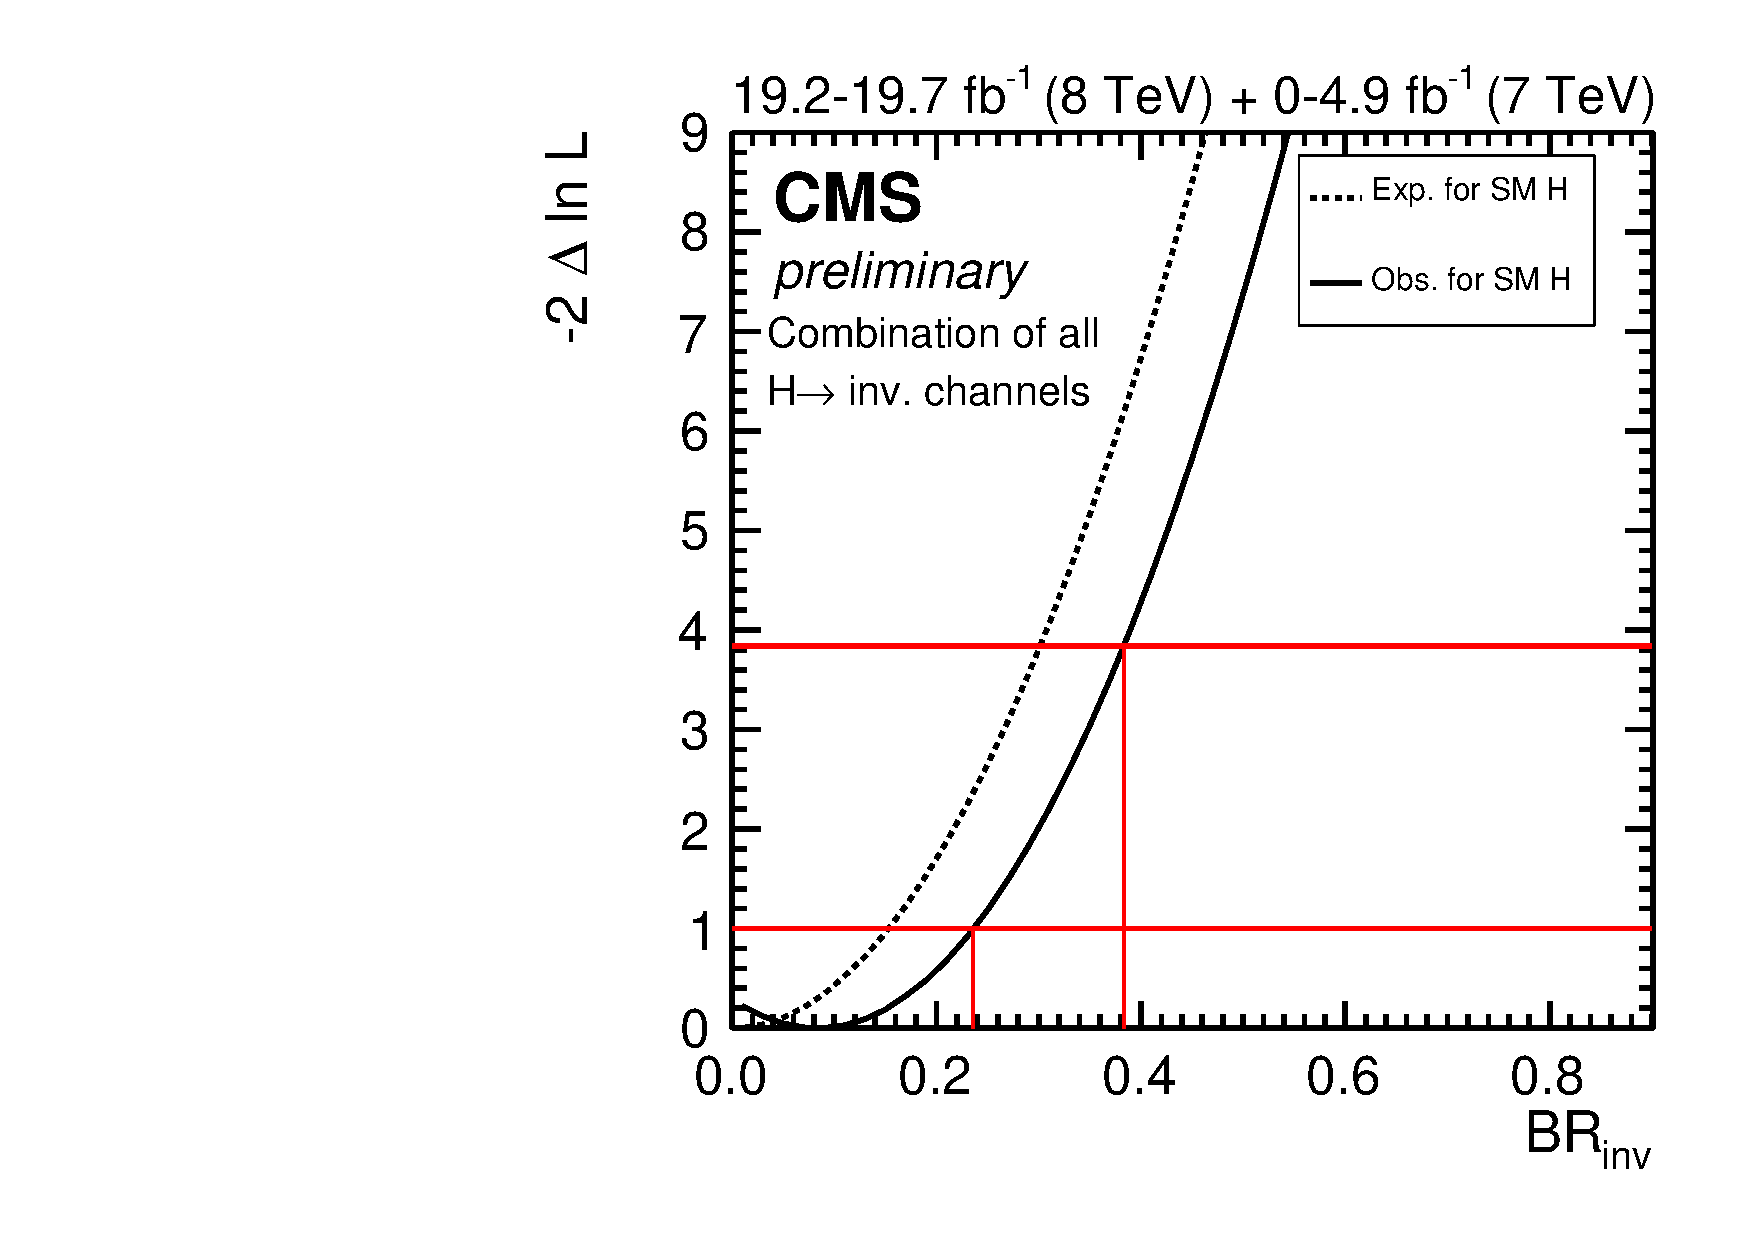
\includegraphics[width=.95\textwidth]{TalkPics/hig15012approval/combscan.pdf}
    \column{.5\textwidth}
    \centering
    \textcolor{red}{For Approval - Additional Material}
    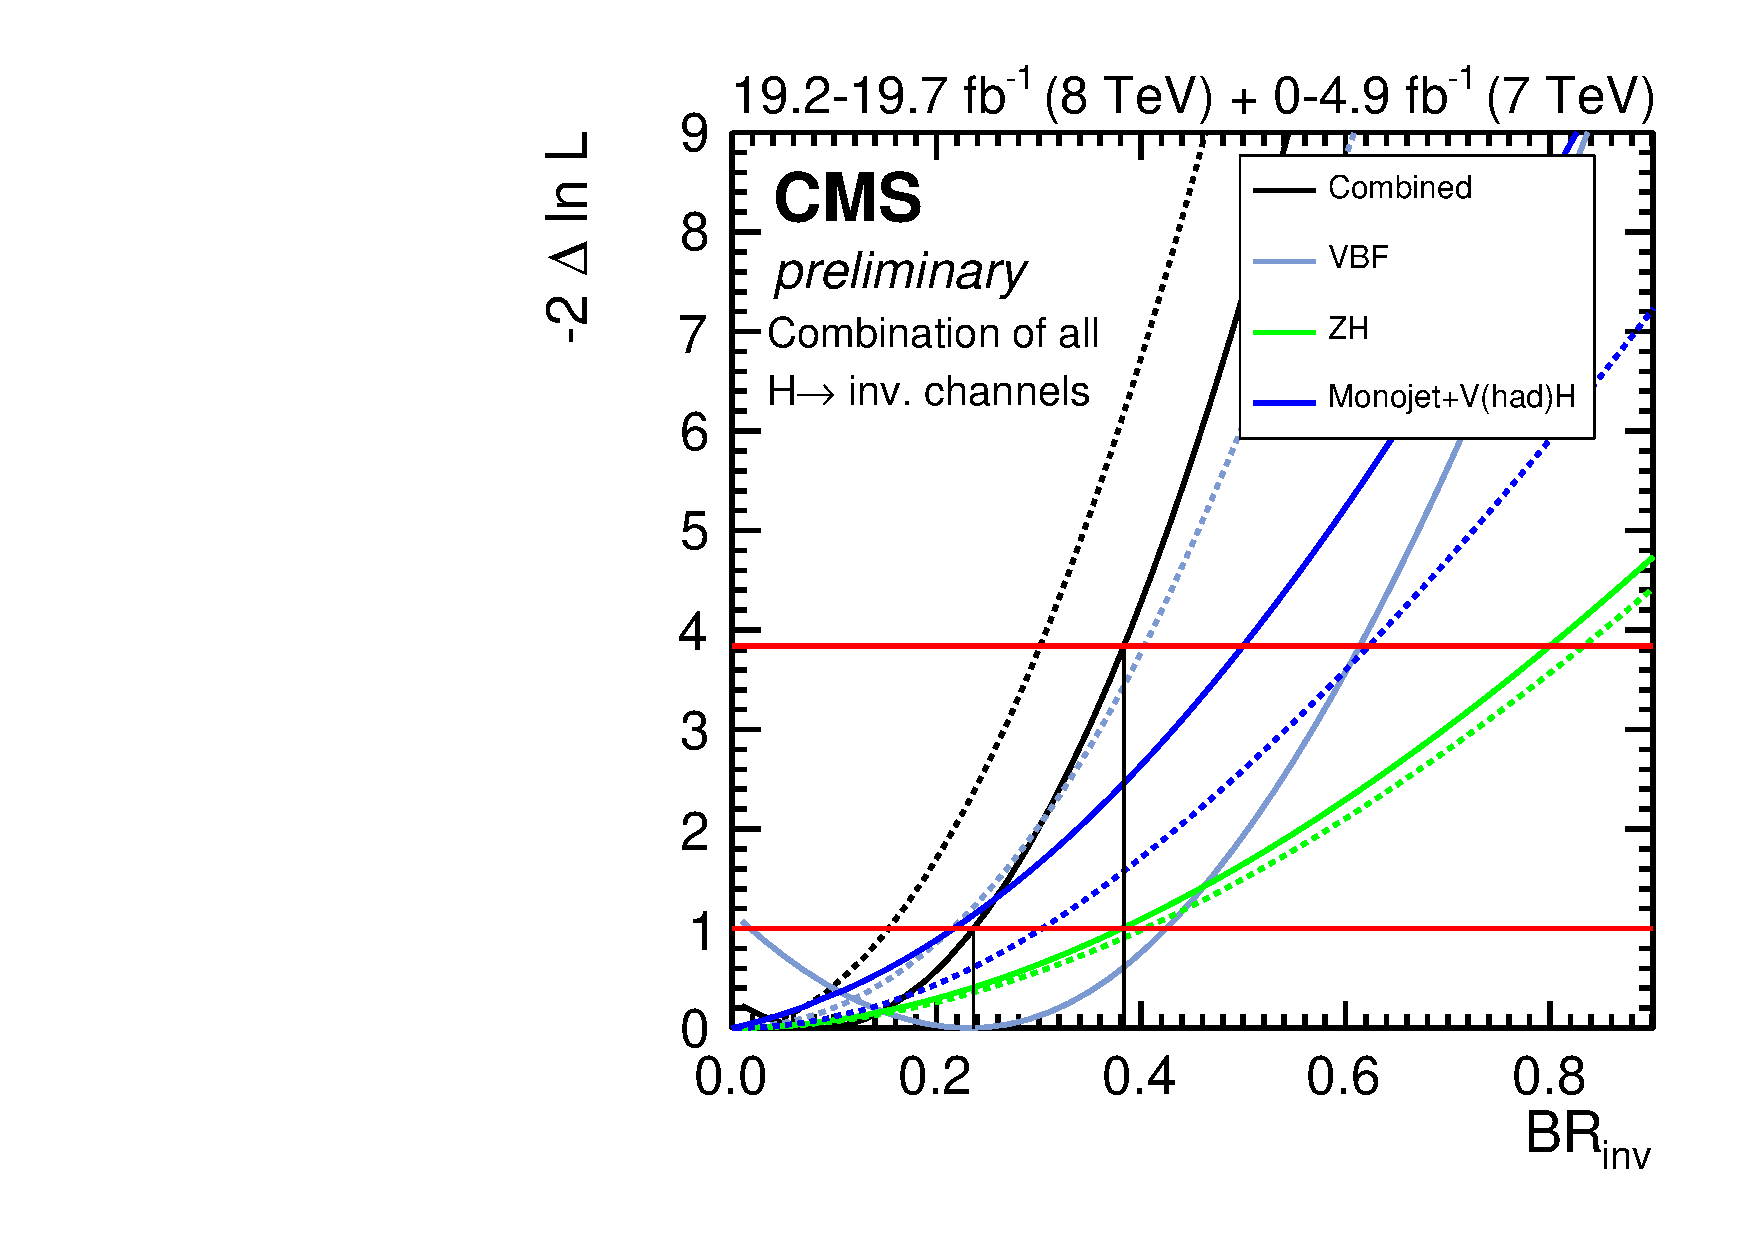
\includegraphics[width=.95\textwidth]{TalkPics/hig15012approval/scanallchannels.pdf}
    \end{columns}
\end{frame}

\begin{frame}
  \frametitle{Likelihood scans}
  \scriptsize
  \begin{columns}
    \column{.5\textwidth}
    \begin{block}{}
      \begin{itemize}
      \item Likelihood scan with statistical errors only also requested by the ARC
      \item Not obvious from Z(bb)H data cards which uncertainties are statistical
      \item[-] Impact of Z(bb)H is small so we froze all its nuisances
      \end{itemize}
    \end{block}
    \column{.5\textwidth}
    \centering
    \includegraphics[width=\textwidth]{TalkPics/hig15012approval/statonlyscan.pdf}
  \end{columns}
\end{frame}

\begin{frame}
  \frametitle{Limits - by production mode tag}
  \centering
  \scriptsize
  \vspace{-.3cm}
  \begin{block}{}
    \begin{itemize}
    \item VBF tagged is VBF analysis
    \item VH-tagged is Z(ll)H + Z(bb)H + boosted and resolved from monojet+V(had)H
    \item ggH-tagged is monojet from monojet+V(had)H
    \end{itemize}
  \end{block}
  \textcolor{red}{For Approval}

  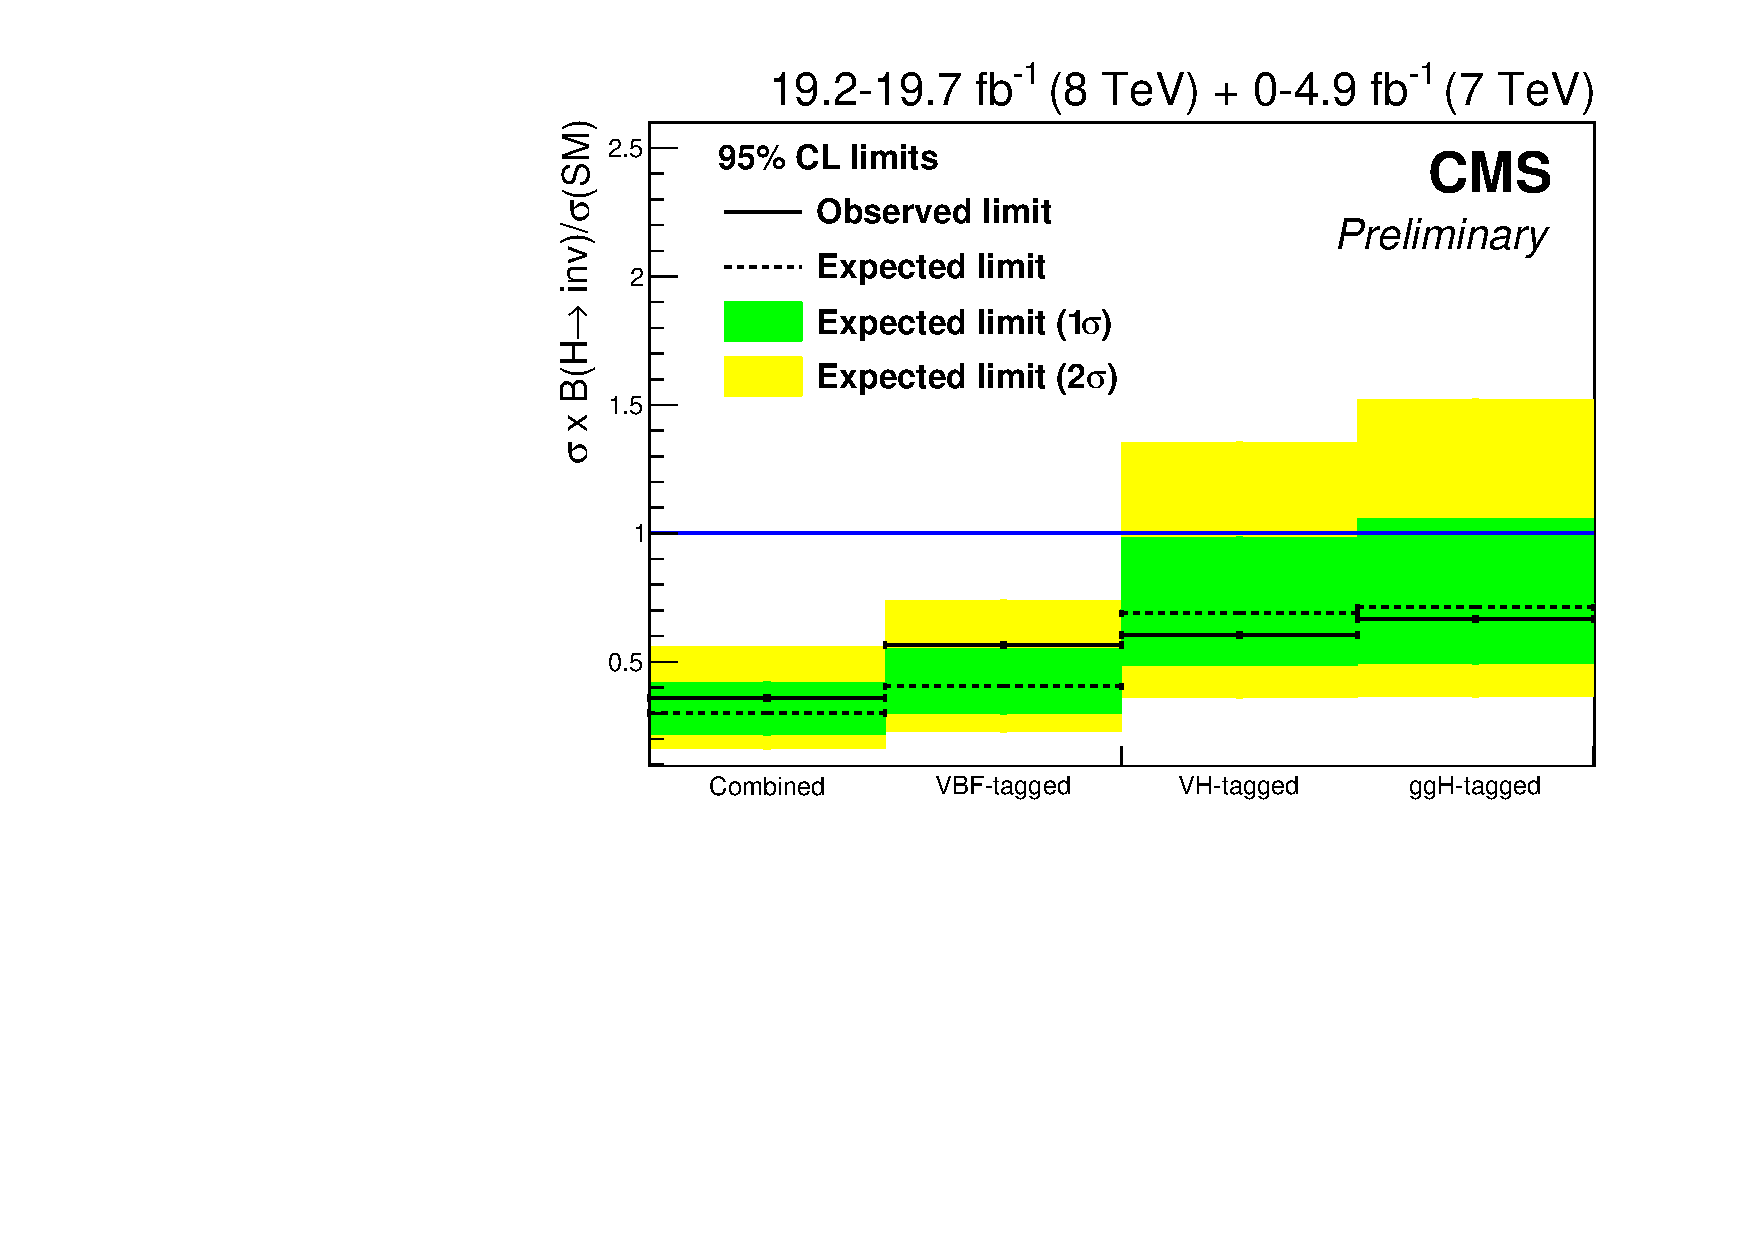
\includegraphics[width=.64\textwidth]{TalkPics/hig15012approval/channellimit.pdf}

\end{frame}

\begin{frame}
  \frametitle{Summary}
  \label{lastframe}
  \begin{block}{}
    \scriptsize
    \begin{itemize}
    \item All CMS Run I H$\rightarrow$invisible analyses have been combined
    \item The observed (expected) 95\% CL upper limit on B(H$\rightarrow$inv) is \textcolor{red}{36} (\textcolor{red}{30})\%
    \item We ask for approval
    \end{itemize}
  \end{block}
  \centering
  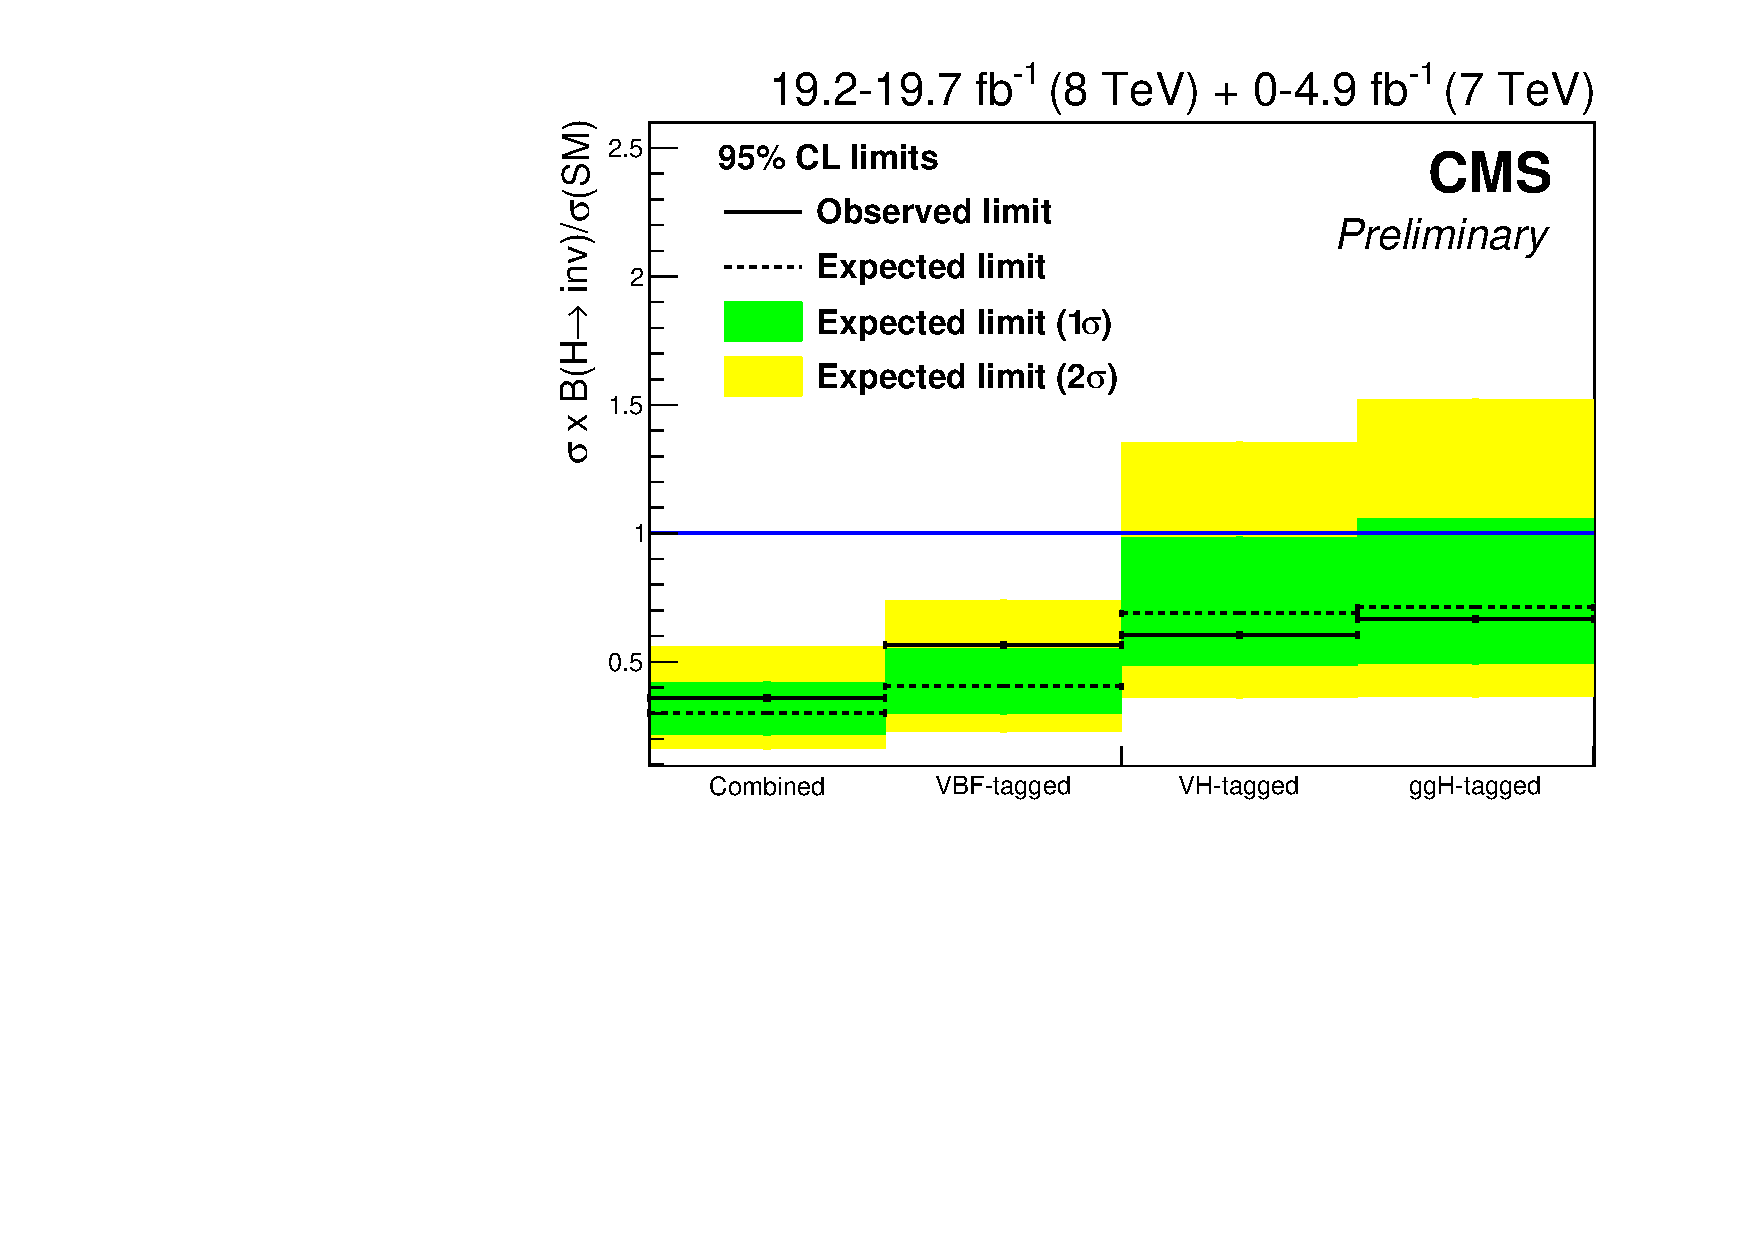
\includegraphics[width=.6\textwidth]{TalkPics/hig15012approval/channellimit.pdf}
\end{frame}

%UPDATED BACKUP
\begin{frame}
  \frametitle{Backup}
\end{frame}

%THEORY MOTIVATION
\begin{frame}
    \frametitle{Why Higgs to Invisible?}
    \vspace{-.2cm}
    \begin{columns}
      \column{.5\textwidth}
      \begin{block}{\scriptsize Experimental motivation}
        \scriptsize
        \begin{itemize}
        \item Current measurements of the 125 GeV Higgs boson are compatible with Standard Model (SM) expectations
        \item[-] large uncertainties can still accommodate significant beyond the SM (BSM) properties
        \item Additional Higgs bosons with exotic decays are not excluded
        \end{itemize}
      \end{block}
      \column{.45\textwidth}
      \hfill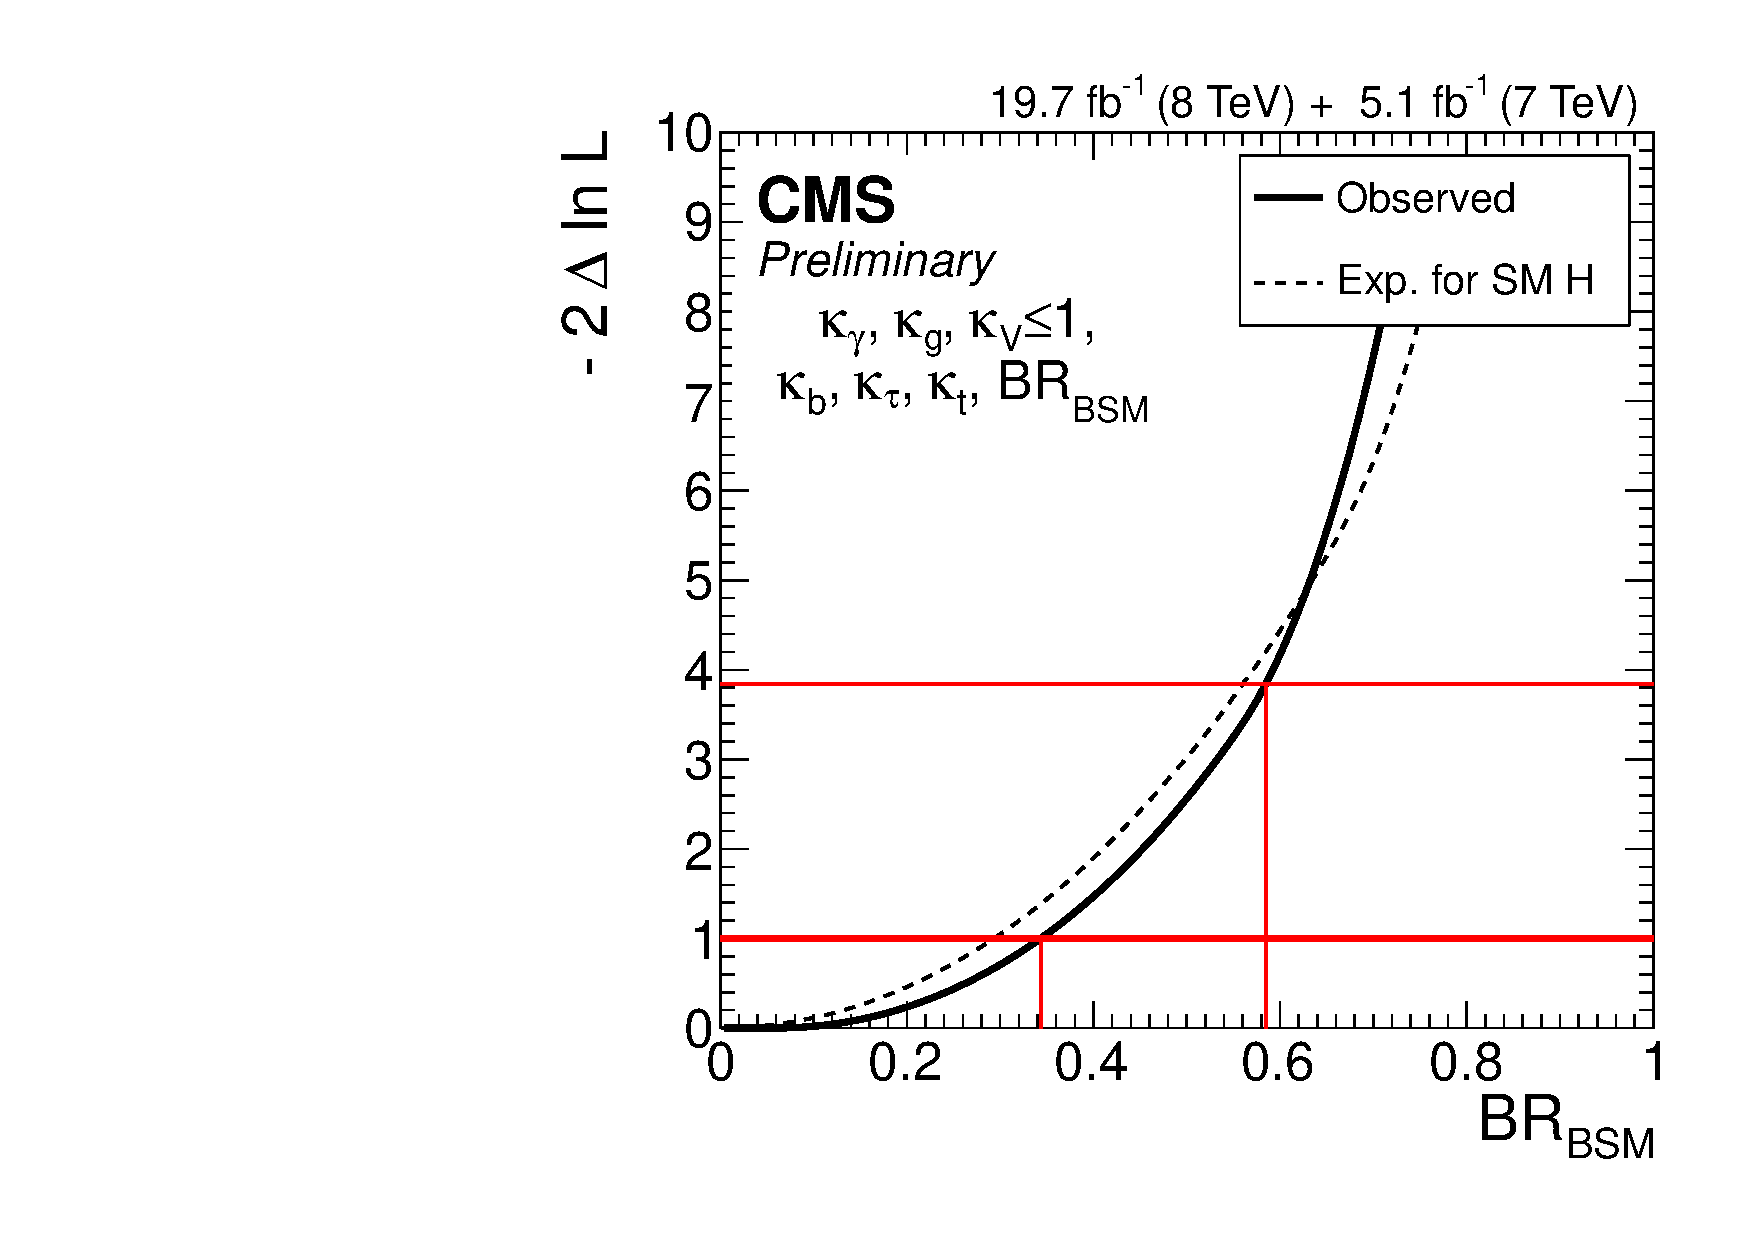
\includegraphics[height=.55\textheight]{TalkPics/panicpics/indirectbrbsm.pdf}
      \column{.05\textwidth}
    \end{columns}
    \begin{columns}
      \column{1.095\textwidth}
      \begin{block}{\scriptsize Theoretical motivation}
        \scriptsize
        \begin{itemize}
        \item Many BSM theories predict Higgs boson decays to invisible final states:
        \item[-] e.g. SUSY, extra dimensions, fourth-generation neutrinos
        \item These final state particles are often dark matter candidates
        \end{itemize}
      \end{block}
    \end{columns}

  \end{frame}

\begin{frame}
  \frametitle{Pulls}
  \scriptsize
  \begin{block}{}
    \begin{itemize}
    \item Usual full table of pulls and post-fit nuisances in AN/2014-206
    \item Generally distributed around their pre-fit values
    \item[-] Apologies for x axis below
    \end{itemize}
  \end{block}
  \centering
  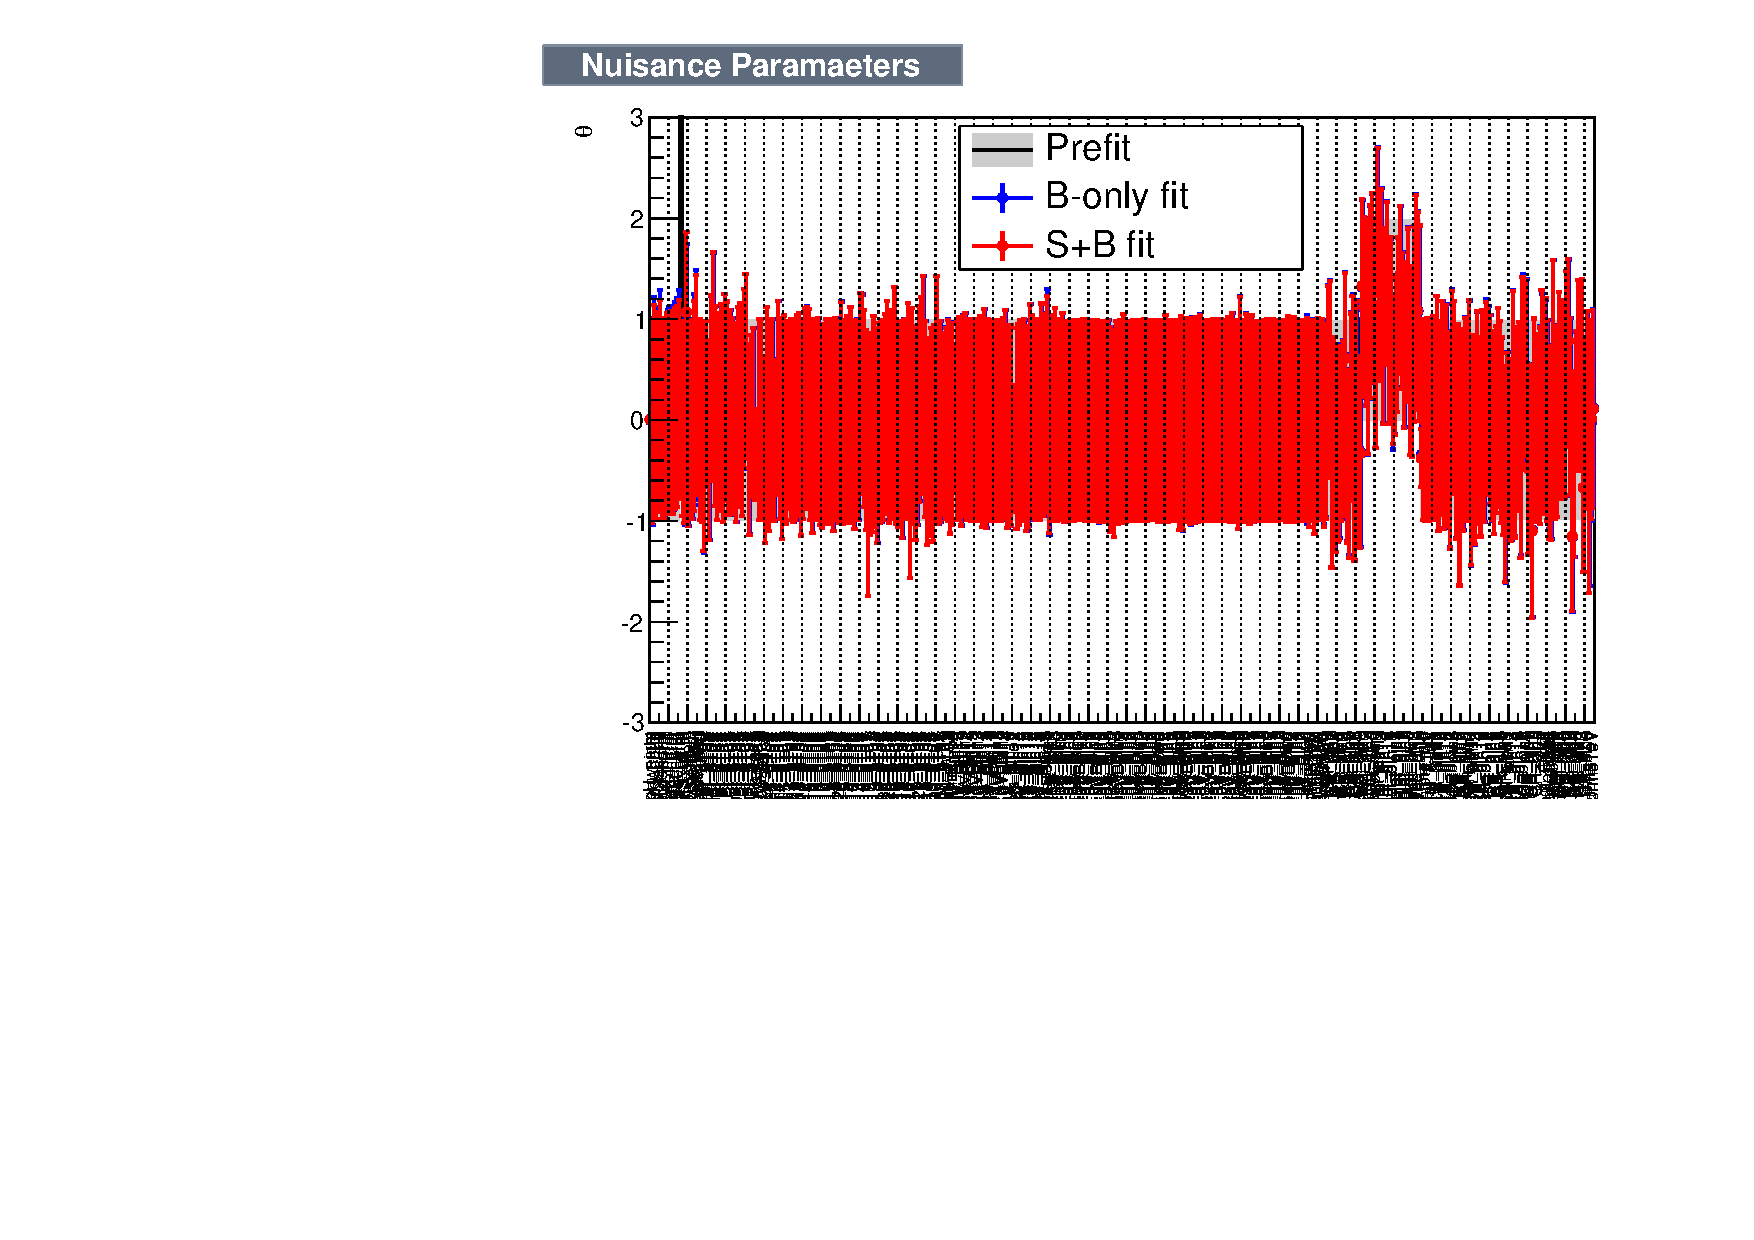
\includegraphics[width=.7\textwidth]{TalkPics/hig15012preapproval/pulls.pdf}

\end{frame}






%ADD OBJECTS INFO
\begin{frame}
  \frametitle{VBF Objects}
  \begin{columns}
    \column{.5\textwidth}
    \vspace{-.3cm}
    \begin{block}{\scriptsize PFMET}
      \scriptsize
      \begin{itemize}
      \item Ignore muons
      \item Type0+1 corrections
      \item Smeared PFMET for MC
      \end{itemize}
    \end{block}
    \vspace{-.3cm}
    \begin{block}{\scriptsize AK5 PFJets}
      \scriptsize
      \begin{itemize}
      \item L1FastJet+L2+L3(+L2L3Residual) JEC
      \item ``Loose'' PF Jet ID
      \item Cleaned with veto leptons
      \item ``Loose'' PU jet ID
      \item Smeared jet collection for MC (JER is smeared to match data)
      \end{itemize}
    \end{block}
    \column{.5\textwidth}
    \vspace{-.3cm}
    \begin{block}{\scriptsize Veto leptons}
      \scriptsize
      \begin{itemize}
      \item loose+PFiso muons $p_{T}>10$ GeV, $|\eta|<2.1$
      \item veto+PFiso electrons $p_{T}>10$ GeV, $|\eta|<2.4$
      \end{itemize}
    \end{block}
    \vspace{-.3cm}
    \begin{block}{\scriptsize Tight leptons}
      \scriptsize
      \begin{itemize}
      \item As veto leptons but ``tight'' ID and $p_{T}>20$ GeV
      \end{itemize}
    \end{block}
    \vspace{-.3cm}
    \begin{block}{\scriptsize Hadronic taus}
      \scriptsize
      \begin{itemize}
      \item $p_{T}>20$ GeV, $|\eta|<2.3$,$d_{Z}<0.2$ cm
      \item Tight ID, discriminant ``byTightCombinedIsolationDeltaBetaCorr3Hits''
      \item Efficiency $\sim$0.55, fake rate 0.02(barrel),0.03(endcap)

      \end{itemize}
    \end{block}
  \end{columns}
\end{frame}


\end{fmffile}
\end{document}
